% autosam.tex
% Annotated sample file for the preparation of LaTeX files
% for the final versions of papers submitted to or accepted for 
% publication in AUTOMATICA.

% See also the Information for Authors.

% Make sure that the zip file that you send contains all the 
% files, including the files for the figures and the bib file.

% Output produced with the elsart style file does not imitate the
% AUTOMATICA style. The style file is generic for all Elsevier
% journals and the output is laid out for easy copy editing. The
% final document is produced from the source file in the
% AUTOMATICA style at Elsevier.

% You may use the style file autart.cls to obtain a two-column 
% document (see below) that more or less imitates the printed 
% Automatica style. This may helpful to improve the formatting 
% of the equations, tables and figures, and also serves to check 
% whether the paper satisfies the length requirements.

% Please note: Authors must not create their own macros.

% For further information regarding the preparation of LaTeX files 
% for Elsevier, please refer to the "Full Instructions to Authors" 
% from Elsevier's anonymous ftp server on ftp.elsevier.nl in the
% directory pub/styles, or from the internet (CTAN sites) on
% ftp.shsu.edu, ftp.dante.de and ftp.tex.ac.uk in the directory
% tex-archive/macros/latex/contrib/supported/elsevier.


%\documentclass{elsart}               % The use of LaTeX2e is preferred.

\documentclass[twocolumn]{autart}    % Enable this line and disable the 
                                     % preceding line to obtain a two-column 
                                     % document whose style resembles the
                                     % printed Automatica style.


\usepackage{graphicx}          % Include this line if your 
                               % document contains figures,
%\usepackage[dvips]{epsfig}    % or this line, depending on which
                               % you prefer.
\usepackage{amsmath,amssymb,amstext,amsfonts,subfigure,bm,dsfont,epsfig,esint,stfloats,graphicx}
\usepackage{cuted}%%\stripsep-3pt
\stripsep -3pt plus 3pt minus 2pt
\usepackage{multicol}
\usepackage{booktabs}
\usepackage{graphicx}

\usepackage{caption}
\usepackage[justification=centering]{caption}

\usepackage{comment}
\usepackage{cite}
\usepackage{algorithmic}
\usepackage{graphicx}
\usepackage{pgfplots}
\usepackage{textcomp}
\usepackage{xcolor}
\usepackage{multirow}
%\usepackage{threeparttable} % to use notes for the table
\usepackage{pifont}
\usepackage{url}
%\usepackage{ninecolors}
\usepackage{tikz}
\usetikzlibrary{patterns}

\usepackage{acronym}
\usepackage{multirow}
\usepackage[flushleft]{threeparttable} % to use notes for the table
\usepackage[T1]{fontenc} % allows the direct use of >, <, = etc.


\usepackage{enumitem}

\usepackage[utf8]{inputenc}
\usepackage{eurosym}

\usepackage{booktabs} % To thicken table lines

\usepackage{url}
\usepackage{threeparttable}
\usepackage{makecell}
\usepackage{pifont}
\usepackage{graphicx}
\usepackage{pgfplots}
\pgfplotsset{compat=newest}
\usepackage{textcomp}
\usepackage{xcolor}
\usepackage{siunitx}

\usepackage{tikz}
\usetikzlibrary{calc,trees,positioning,arrows,chains,shapes.geometric,%
    decorations.pathreplacing,decorations.pathmorphing,shapes,%
    matrix,shapes.symbols}

\tikzset{
>=stealth',
  punktchain/.style={
    rectangle, 
    rounded corners, 
    % fill=black!10,
    draw=black, very thick,
    text width=10em, 
    minimum height=3em, 
    text centered, 
    on chain},
  line/.style={draw, thick, <-},
  element/.style={
    tape,
    top color=white,
    bottom color=blue!50!black!60!,
    minimum width=8em,
    draw=blue!40!black!90, very thick,
    text width=10em, 
    minimum height=3.5em, 
    text centered, 
    on chain},
  every join/.style={->, thick,shorten >=1pt},
  decoration={brace},
  tuborg/.style={decorate},
  tubnode/.style={midway, right=2pt},
}


\begin{document}

\begin{frontmatter}
%\runtitle{Insert a suggested running title}  % Running title for regular 
                                              % papers but only if the title  
                                              % is over 5 words. Running title 
                                              % is not shown in output.

\title{11111111\thanksref{footnoteinfo}} % Title, preferably not more 
                                                % than 10 words.

\thanks[footnoteinfo]{This paper was not presented at any IFAC 
meeting. Corresponding author M.~T.~Cicero. Tel. +XXXIX-VI-mmmxxi. 
Fax +XXXIX-VI-mmmxxv.}

\author[Paes1tum]{Marcus Tullius Cicero}\ead{cicero@senate.ir},    % Add the 
\author[Rome]{Julius Caesar}\ead{julius@caesar.ir},               % e-mail address 
\author[Baiae]{Publius Maro Vergilius}\ead{vergilius@culture.ir}  % (ead) as shown

\address[Paestum]{Buckingham Palace, Paestum}  % Please supply                                              
\address[Rome]{Senate House, Rome}             % full addresses
\address[Baiae]{The White House, Baiae}        % here.

          
\begin{keyword}                           % Five to ten keywords,  
LOI; switched system; neutral system.               % chosen from the IFAC 
\end{keyword}                             % keyword list or with the 
                                          % help of the Automatica 
                                          % keyword wizard


\begin{abstract}                          % Abstract of not more than 200 words.
abstract
\end{abstract}

\end{frontmatter}

\section{Introduction}

Recently,a novel L-K functional based on the Partial-Integral operator.The new L-K functional denotes the
complete L-K functional by inner product.For the Linear Time Delay system with time-invariant delay,we can 
obtain less conservative results even necessary and sufficient results.

(SOS)provide a computationally tractable test for Zeno stability in hybrid systems with semi-algebraic 
guard sets.develop a polynomial-time algorithm for construciton of the Lyapunov-like funtion proposed
in (23) and (24).extend this method to the verification of Zeno stability for system with parameetric 
uncertainly.

(wangyibo)A complete quadratic L-K functional was built in theform of an inner product of the PI operator, which has 
the potential to obtain accurate stability conditions.The novel stability criteria for the multiarea LFC 
systems with time delays were proposed in this article, which were less conservative than existing literature. Furthermore, the relationships between controller 
parameters and delay margins were further studied

(wushuangshuang) use PIE-based methods to analyze stability and $H_{\infty}$ performance problem of linear 
TDSs with uncertain delays.

(chaitanya Murti) provide  a computationally tractable test for Zeno stability in hybrid system with semi-algebraic 
guard sets.use Sum-of-Squares to find a convex approach for construciton of Lyapunov functions for Zeno stability.

(PIETOOLS)present PIETOOLS matlab toolbox for construciton and handling of Partial Integral(PI) operator.After several refinements, PIETOOLS comes to the latest version of 2022.
In the 2022 version, user manuals and many demos were added.Simulations of this paper based on PIETOOLS2022. 

(Minimal Differential Difference)
Propose a an algorithm for constructing minimal DDF relization of DDE systems. The algorithm can dramatically reduce the computational 
complexity of analysis and control problems for delayed networks.And it extended this result to a algorithm for minimal DDF relizations
of DDFs-thus also solving the problem of inefficient DDF representing of NDSs.

The LOI method in (article Representation) is further extended to the neutral system by (Representation),comparing with the method used by Delay-Dependent Stability for 
Load Frequency Control System via Linear Operator Inequality, the new method can 
convert not only multiple time-delay system but also the nuetral delay system(NDS) 
even the neutral system with Integral term.
provide formulae for conversion between representations under which solutions are equivalent.

The LOI method in (article Representation) was already further extended to the neutral system by (Representation),
however, those theorems proposed for linear time delay system(muti delay?multi-delay system) have not been extended to neutral system.

In neutral delay system,the delay not only exsit in the state of s but also exsit in the derivative 
of state.The delay in (derivative term) calls neutral delay.

The traditional method for linear neutral switched system globally stability
constructing Lyapunov function integral term with exponential coefficient.It is necessary to ensure that after the derivation 
and the addition of the original function, the complex quadratic integral term can be eliminated and only the simple first 
integral term can be left. Finally, a very complex matrix negative definite condition is obtained by Jensen inequality and the 
global stability condition of the switched system is obtained by using the hypothesis condition.

In this article,we use the extended conversion formulae to convert NDS to PIE.The previous LOI criterion which can only deal with constant delay 
systems is extended to neutral delay systems.In addition, the complete L-K functional based on inner product is applied to neutral switched systems 
to obtain a simpler and less conservative global stability criterion.

\section{Problem formulation and preliminaries}

Consider a neutral switched system described by the following equation:
%See \cite{Abl:56}, \cite{AbTaRu:54}, \cite{Keo:58} and 
%\cite{Pow:85}.
\begin{equation} \label{e1}
    \begin{aligned}
        &\dot{x}(t) = A_{\sigma(t)}x(t) + B_{\sigma(t)}x(t-r) \\
        & \qquad \qquad \qquad \qquad + C_{\sigma(t)}\dot{x}(t-h)+ D_{\sigma(t)}u(t) \\
        &x(\theta) = \Psi(\theta),\forall \theta \in [-H,0],H = max\{t,h\}
    \end{aligned}
\end{equation}

where $x(t) \in R^{n}$ is the state,$u(t) \in R^{p}$ denote the system state and control input.$\sigma(t):[0,+\infty) \rightarrow \mathcal{P}$ 
is a piecewise constant function denote switching signal. $h$ and $r$ are the state delay and neutral delay.
$\Psi(\theta)$ is a initial vector function on $[-H,0]$.

The Zeno and impulsive conditions are assumed to be excluded consideration.The switching sequence is expressed as 
\begin{equation} \label{e1}
    \begin{aligned}
        \aleph _{p} &= \{(\sigma(t_{0}),t_{0}),\ldots (\sigma(t_{k}),t_{k}),\ldots\\
        & \qquad |\sigma(t_{k}) \in \mathcal{P},k = 0,1,\ldots\}
    \end{aligned}
\end{equation}
where $t_{0}$ is the initial time and  $t_{k}$ is the switching instant. The $\sigma(t_{k})$th subsystem is active when $t \in [t_{k},t_{k+1})$. 
%For $i \in \{\mathcal{P},Ai, Bi, Ci, Di\}$ are known real constant matrices of appropriate dimensions.

Considering the asynchronous switching, the candidate controller presented in the form of 
\begin{equation} \label{e1}
    \begin{aligned}
        u(t) = K_{\sigma(t-\tau(t))}x(t)
    \end{aligned}
\end{equation}
where $\tau(t)$ Represents the switching delay satisfying $0 \textless \tau(t) \textless \tau_{d} \textless t_{k+1}-t_{k},\forall k \in \mathbb{N} $.

Operator

%算子运算说明
%参考wangyibo



If we also do not consider the output $y(t)$,we can convert Equation (1) to standard NDS(Neutral Delay System) (4) by Lemma (NDStoDDF)
\begin{equation}
    \begin{aligned}
        \begin{bmatrix}
            \dot{x}(t) \\
            z(t) \\
            y(t) 
        \end{bmatrix} &=\begin{bmatrix}
            A_{\sigma(t)} & 0 & D_{\sigma(t)}\\
            0 & 0 & 0\\
            0 & 0 & 0
        \end{bmatrix}\begin{bmatrix}
            x(t) \\
            w(t) \\
            u(t) 
        \end{bmatrix} \\ 
        &+ \quad \begin{bmatrix}
            B_{\sigma(t)} & 0 & 0 & 0\\
            0 & 0 & 0 & 0\\
            0 & 0 & 0 & 0
        \end{bmatrix} \begin{bmatrix}
            x(t-r) \\
            w(t-r) \\
            u(t-r) \\
            \dot{x}(t-r)
        \end{bmatrix} \\
        &+ \qquad \begin{bmatrix}
            0 & 0 & 0 & C_{\sigma(t)}\\
            0 & 0 & 0 & 0\\
            0 & 0 & 0 & 0
        \end{bmatrix} \begin{bmatrix}
            x(t-h) \\
            w(t-h) \\
            u(t-h) \\
            \dot{x}(t-h)
        \end{bmatrix}
    \end{aligned}
\end{equation}

\begin{assum}
    For any subsystem i switching to j where $i,j \in \mathcal{P}$, there exsits a scalar $\mu_{ij} \textgreater 0$, the following inequality holds:
    \begin{equation}
            \begin{aligned}
                \setlength{\arraycolsep}{0.9pt}
                V_{j}(x(t)) \le \mu_{ij}V_{i}(x(t)) \quad \forall x(t) \in R^{n}
            \end{aligned}
        \end{equation}
    \end{assum}

\begin{defn}
    Let $N_{\sigma}(t)$ denote the switching times in the time interval $(0,t)$,then we define the h-frequency of switching at $t$ as
    \begin{equation}
        \begin{aligned}
            \setlength{\arraycolsep}{0.9pt}
            v_{t}(t) := \frac{N_{\sigma(t)}}{h(t)}
        \end{aligned}
    \end{equation}
\end{defn}

\begin{defn}
We divide the time interval into the mismatched period $\mathcal{M}_{1}$ and matched period $\mathcal{M}_{2}$.

Let $\mathcal{P}_{m1}$ denote the index set systems during the mode-identifying period or mismatched period. Meanwhile, denote
$\mathcal{P}_{m2}^{s}$, $\mathcal{P}_{m2}^{u} \in \mathcal{P}_{m2}$ as the stable and unstable indices sets during the normal-working period, respectively. Namely,
\begin{equation}
    \begin{aligned}
        \setlength{\arraycolsep}{0.9pt}
        &\mathcal{P}_{m1} = \{i \in \mathcal{P} | \sigma(t) = i,\\
        &\qquad \qquad \qquad \qquad  \forall t \in [t_{k},t_{k}+\tau(t_{k})),k = 0,1,\ldots\}\\
        &\mathcal{P}_{m1} = \{i \in \mathcal{P} | \sigma(t) = i,\\
        &\qquad \qquad \qquad \qquad\forall t \in [t_{k}+\tau(t_{k},t_{k})),k = 0,1,\ldots\}
    \end{aligned}
\end{equation}
Clearly, it holds that $\mathcal{P} = \mathcal{P}_{m1} = \mathcal{P}_{m2} = \mathcal{P}_{m2}^{s}\bigcup \mathcal{P}_{m2}^{u}$
\end{defn}

\begin{figure}[htbp]
    \centering
    \includegraphics[width=0.47\textwidth,height=0.168\textwidth]{2_1.png}
    \caption{A S}
    \end{figure} 

\begin{rmk}
    reamrk1
\end{rmk}


\begin{defn}
    
    Define the kth holding time of a switching
    signal $\sigma$ in the matched period as
    \begin{equation}
        \begin{aligned}
            \setlength{\arraycolsep}{0.9pt}
            S_{k+1} = t_{k+1} - (t_{k}+\tau(t_{k})), \quad k = 0,1\ldots 
        \end{aligned}
    \end{equation}
    Then, for each $j \in \mathcal{P}$, define the h-frequency of activation of subsystem $j$ in mismatched period as
    \begin{equation}
        \begin{aligned}
            \setlength{\arraycolsep}{0.9pt}
            \eta^{h}_{1}(j,t) := \sum_{i:\sigma(t_{i}) = j}\frac{\tau_{t_{i}}}{h(t)}, \quad t\textgreater 0
        \end{aligned}
    \end{equation}
    In matched period, the corresponding h-frequency of activation of subsystem $j$ is defined as
    \begin{equation}
        \begin{aligned}
            \setlength{\arraycolsep}{0.9pt}
            \eta^{h}_{2}(j,t) := \sum_{i:\sigma(t_{i}) = j}\frac{S_{i+1}}{h(t)}, \quad t\textgreater 0
        \end{aligned}
    \end{equation}
    Let $E(\mathcal{P})$ be the set for admissible switch from subsystem $m$ to subsystem $n$, $\forall m, n \in \mathcal{P}$, which is represented by a
    sequential pair $(m,n)$. For each pair $(m,n) \in E(\mathcal{P})$, we define the transition frequency from the $m$th subsystem to the $n$th
    subsystem as
    \begin{equation}
        \begin{aligned}
            \setlength{\arraycolsep}{0.9pt}
            \rho_{mn}(t) := \frac{\# \{m \rightarrow n\}}{N_{\sigma}} , \quad t \textgreater 0
        \end{aligned}
    \end{equation}
    where$\# \{m\rightarrow n\}_{t}$ is the transition number from subsystem $m$ to subsystem $n$ in the time interval $[0,t)$
    
    Now, define the asymptotic upper density of $v_{h}$,$\rho_{mn}$ as
    \begin{equation}
        \begin{aligned}
            \setlength{\arraycolsep}{0.9pt}
            \hat{v}_{h} := \lim_{t \rightarrow +\infty} \sup v_{h}(t)
        \end{aligned}
    \end{equation}
    \begin{equation}
        \begin{aligned}
            \setlength{\arraycolsep}{0.9pt}
            \hat{\rho}_{mn} := \lim_{t \rightarrow +\infty} \sup \rho_{mn}(t)
        \end{aligned}
    \end{equation}

    Similarly, the asymptotic upper densities of $\eta_{1}^{h}(j,t)$,$\eta_{2}^{h}(j,t)$ are defined as
    \begin{equation}
        \begin{aligned}
            \setlength{\arraycolsep}{0.9pt}
            \hat{\eta}^{h}_{1}(j) := \lim_{t \rightarrow +\infty} \sup \eta_{1}^{h}(j,t)
        \end{aligned}
    \end{equation}
    \begin{equation}
        \begin{aligned}
            \setlength{\arraycolsep}{0.9pt}
            \hat{\eta}^{h}_{2}(j) := \lim_{t \rightarrow +\infty} \sup \eta_{2}^{h}(j,t)
        \end{aligned}
    \end{equation}

    In addition, we also give the definition of asymptotic lower densities of $\eta_{2}^{h}(j,t)$ as
    \begin{equation}
        \begin{aligned}
            \setlength{\arraycolsep}{0.9pt}
            \breve{\eta}^{h}_{2}(j) := \lim_{t \rightarrow +\infty} \inf \eta_{2}^{h}(j,t)
        \end{aligned}
    \end{equation}
\end{defn}



Z inner produced
%Z内积定义 用Peet那个文章里复杂的那个
\begin{equation}
    \begin{aligned}
        \setlength{\arraycolsep}{0.9pt}
        \left<  \begin{bmatrix}
            y\\
            \psi_{i}
        \end{bmatrix},\begin{bmatrix}
            x\\
            \phi_{i}
        \end{bmatrix} \right>_{Z_{m,n,K}} =y^{T}x + \int_{-1}^{0}\psi_{i}(s)^{T}\phi_{i}(s)ds
    \end{aligned}
\end{equation}

To establish the main result of this paper, we review four useful lemmas that will be used in the proof of this paper .
%lemma yibo wang
\begin{lem}
    [c]For given time delays $\tau_{i}(i=0,1,\cdots N)$ the system $\mathcal{T}\dot{x}_{f}(t) = \mathcal{A}x_{f}(t)$ is asymptotically stable 
    if there exsit a positive,self-adjoint PI operator $\mathcal{P}:=\mathcal{P}\begin{bmatrix}
        P,&Q_{1}\\
        Q_{2},&\{R_{i}\}
    \end{bmatrix}$ such that the following inequality holds:
    \begin{equation}
        \mathcal{T}^{*}\mathcal{P}\mathcal{A}+\mathcal{A}^{*}\mathcal{T}\mathcal{P} \textless 0
    \end{equation}
\end{lem}
    The proof of lemma 1 will be found in Appendixes

\begin{lem}[c]
    then we get the standard DDF form
\begin{equation}
    \begin{aligned}
        \begin{bmatrix}
            \dot{x}(t) \\
            z(t) \\
            y(t) \\
            r_{i}(t)
        \end{bmatrix} & = \begin{bmatrix}
            A_{\sigma(t)} & 0 & D_{\sigma(t)}\\
            0 & 0 & 0\\
            0 & 0 & 0\\
            C_{ri} & B_{r1i} & B_{r2i}
        \end{bmatrix}\begin{bmatrix}
            x(t) \\
            w(t) \\
            u(t) 
        \end{bmatrix} 
        +  \begin{bmatrix}
            B_{v} \\
            D_{1v} \\
            D_{2v} \\
            D_{rvi}
        \end{bmatrix}v(t)\\
        v(t) &= C_{v1}r_{1}(t-r) + C_{v2}r_{2}(t-h)
    \end{aligned}
\end{equation}
\end{lem}

\begin{lem}
    
And then we try to (cite Representation of Networks and Systems with Delay:DDEs, DDFs, ODE-PDEs and PIEs) convert standard DDF form Equation (7) to PIE from Equation (8) 
\begin{equation}
    \begin{aligned}
        \setlength{\arraycolsep}{0.9pt}
        \mathcal{T}\dot{\bold{x}}+\mathcal{B}_{T_{2}}\dot{u} = \mathcal{A}\bold{x}+\mathcal{B}_{2}u
    \end{aligned}
\end{equation}
\begin{equation}
    \begin{aligned}
        \setlength{\arraycolsep}{0.9pt}
        \bold{x(t)} := \begin{bmatrix}
            x(t) \\
            \Phi(t,.)
        \end{bmatrix}\nonumber
    \end{aligned}
\end{equation}
\end{lem}
remark?
It should be noticed the difference between $\bold{x}$ and $x$.
The reason why $\bold{x}$ terms and $x$ terms can be added up is that there is no difference
for the operator $\mathcal{B}_{T_{2}}$ to dual with $\bold{x}$ and $x$.

remark
$\mathcal{B}_{T_{2}}$,$B_{2}$ was minimalized by converting program in PIETOOLS2022.  




And then (cite Representation of Networks and Systems with Delay:DDEs, DDFs, ODE-PDEs and PIEs) ,we can convert standard NDS form Equation (3) to DDF(Differential Difference Equations) form Eqution (7) by Eqution (4)

%lemma3 lemma4
%Conversion Formula from NDS to DDF LEMMA2
\begin{figure*}[hb] %hb代表放在文章底部,%ht为放在文章顶部 
    \flushleft
    {\noindent}	 \rule[-10pt]{17.5cm}{0.05em}\\
    \vspace{1.5em}
    \text{Conversion Formula from NDS to DDF:}
    %\centering
    \begin{equation}
        \begin{aligned}
            D_{rvi} &= 
            \begin{bmatrix}
                0 & 0 & 0 \\
                0 & 0 & 0 \\
                0 & 0 & 0 \\
                I & 0 & 0
            \end{bmatrix}       ,    & [C_{ri} \space B_{r1i} \space B_{r2i}] &= 
                                        \begin{bmatrix}
                                            I_{n} & 0 & 0 \\
                                            0 & I_{m} & 0 \\
                                            0 & 0 & I_{p} \\
                                            A_{0} & 0 & B_{2}
                                            \end{bmatrix}  ,                           \qquad & I_{n+q+r}&= 
                                                                                        \begin{bmatrix}
                                                                                            B_{v} \\
                                                                                            D_{1v} \\
                                                                                            D_{2v} 
                                                                                        \end{bmatrix}\ \\
            C_{vi} &= 
            \begin{bmatrix}
                A_{i} & 0 & B_{2i} & E_{i} \\
                0 & 0 & 0 & 0\\
                0 & 0 & 0 & 0\\
                0 & 0 & 0 & 0
            \end{bmatrix}  ,              & C_{vdi}(s) &= 0 
        \end{aligned}
    \end{equation}
\end{figure*}

%Conversion Formula from ODE-PDE to DDF to PIE(1) LEMMA4
\begin{figure*}[hb] %hb代表放在文章底部,%ht为放在文章顶部 
    \flushleft
    \text{Conversion Formula from ODE-PDE to DDF to PIE part1:}
\begin{equation}
    \begin{aligned}
        &\mathcal{A} = \mathcal{P} 
            \begin{bmatrix}
                A_{0} & A \\
                0 & \{I_{\tau},0,0\} 
            \end{bmatrix} ,\quad &\mathcal{T} = \mathcal{P} 
            \begin{bmatrix}
                I & 0 \\
                T_{0} & \{0,T_{a},T_{b}\} 
            \end{bmatrix},\quad &\mathcal{B}_{T_{1}} = \mathcal{P} 
            \begin{bmatrix}
                0 & \varnothing \\
                T_{1} & \{\varnothing\} 
            \end{bmatrix} ,\quad &\mathcal{B}_{T_{2}} = \mathcal{P} 
            \begin{bmatrix}
                0 & \varnothing \\
                T_{2} & \{\varnothing\} 
            \end{bmatrix},\\
        &\mathcal{B}_{1} = \mathcal{P} 
        \begin{bmatrix}
            \bold{B_{1}} & \varnothing \\
            0 & \{\varnothing\} 
        \end{bmatrix},\quad &\mathcal{B}_{2} = \mathcal{P} 
        \begin{bmatrix}
            \bold{B_{2}} & \varnothing \\
            0 & \{\varnothing\} 
        \end{bmatrix},\quad &\mathcal{C}_{1} = \mathcal{P} 
        \begin{bmatrix}
            \bold{C_{10}} & \bold{C_{11}} \\
            \varnothing & \{\varnothing\} 
        \end{bmatrix}, \quad &\mathcal{C}_{2} = \mathcal{P} 
        \begin{bmatrix}
            \bold{C_{20}} & \bold{C_{21}} \\
            \varnothing & \{\varnothing\} 
        \end{bmatrix}
    \end{aligned}
\end{equation}
\vspace{1.5em}
{\noindent}	 \rule[-10pt]{17.5cm}{0.05em}\\
\end{figure*}

%ODE-PDE to DDF to PIE(2)
\begin{figure*}[htb]
    \flushleft
    {\noindent}	 \rule[-10pt]{17.5cm}{0.05em}\\
    \vspace{1.5em}
    \text{Conversion Formula from ODE-PDE to DDF to PIE part2:}
    \begin{equation}
        \begin{aligned}
            &\hat{C}_{vi} = C_{vi},    \quad \quad \quad \quad  D_{I} = 
                                            \begin{bmatrix}
                                                (I-\sum_{i=1}^{K}C_{vi}D_{rvi})^{-1} & 0 & 0 \\
                                                0 & 0 & 0 \\
                                                0 & 0 & I
                                            \end{bmatrix}  ,            \\
            &C_{Ii} = -D_{I}C_{vi} = \begin{bmatrix}
                -(I-\sum_{i=1}^{K}E_{i})^{-1}A_{i} & 0 & -(I-\sum_{i=1}^{K}E_{i})^{-1}B_{2i} & -(I-\sum_{i=1}^{K}E_{i})^{-1}E_{i} \\
                0 & 0 & 0 & 0\\
                0 & 0 & 0 & 0\\
                0 & 0 & 0 & 0
                \end{bmatrix}
                ,           \\   
            &[T_{0} \quad T_{1} \quad T_{2}] = \begin{bmatrix}
                C_{r1}+D_{rv1}C_{vx} & C_{r1}+D_{rv1}D_{vw}  & C_{r1}+D_{rv1}D_{vu}  \\
                C_{r2}+D_{rv2}C_{vx} & C_{r2}+D_{rv2}D_{vw}  & C_{r2}+D_{rv2}D_{vu}  \\
                \vdots & \vdots & \vdots \\
                C_{rK}+D_{rvK}C_{vx} & C_{rK}+D_{rvK}D_{vw}  & C_{rK}+D_{rvK}D_{vu}   
            \end{bmatrix},\\
            &C_{r1}+D_{rv1}C_{vx} = 
            \begin{bmatrix}
            I_{n}    \\
            0        \\
            A_{0}+(I-\sum_{i=1}^{K}E_{i})^{-1}(\sum_{i=1}^{K}(A_{i}+E_{i}A_{0})
            \end{bmatrix},T_{a}(s,\theta) = 
            \begin{bmatrix}
                D_{rv1}C_{I1} & D_{rv1}C_{I2} & \dots & D_{rv1}C_{IK}   \\
                D_{rv2}C_{I1} & D_{rv2}C_{I2} & \dots & D_{rv2}C_{IK}        \\
                \vdots & \vdots & \vdots & \vdots\\ 
                D_{rvK}C_{I1} & D_{rvK}C_{I2} & \dots & D_{rvK}C_{IK}
            \end{bmatrix},\\
            &[C_{vx} \quad D_{vw} \quad D_{vu}] = \begin{bmatrix}
                (I-\sum_{i=1}^{K}E_{i})^{-1}(\sum_{i=1}^{K}(A_{i}+E_{i}A_{0})  & (I-\sum_{i=1}^{K}E_{i})^{-1}(E_{i}B_{1}) & (I-\sum_{i=1}^{K}E_{i})^{-1}(E_{i}B_{2}) \\
                0 &  0 & 0\\
                0 &  0 & 0
            \end{bmatrix},\\
            &D_{rv1}C_{I1} = 
            \begin{bmatrix}
                0 & 0 & 0 & 0   \\
                0 & 0 & 0 & 0          \\
                0 & 0 & 0 & 0  \\ 
                -(I-\sum_{i=1}^{K}E_{i})^{-1}A_{1} & 0 & -(I-\sum_{i=1}^{K}E_{i})^{-1}B_{21} & -(I-\sum_{i=1}^{K}E_{i})^{-1}E_{1}
            \end{bmatrix},\\
            &T_{b}(s,\theta) = -I_{\sum_{i}p_{i}} + T_{a}(s,\theta) = \begin{bmatrix}
                                                                    -I & 0 & 0 & 0   \\
                                                                    0 & -I & 0 & 0          \\
                                                                    0 & 0 & -I & 0  \\ 
                                                                    -(I-\sum_{i=1}^{K}E_{i})^{-1}A_{1} & 0 & -(I-\sum_{i=1}^{K}E_{i})^{-1}B_{21} & -I-(I-\sum_{i=1}^{K}E_{i})^{-1}E_{1}
                                                                \end{bmatrix},\\
            &I_{\tau} = 
            \begin{bmatrix}
            \frac{1}{\tau_{1}}I_{p1} & 0 & 0 & 0   \\
            0 & \frac{1}{\tau_{2}}I_{p2} & 0 & 0          \\
            0 & 0 &\ddots & 0  \\ 
            0 & 0 & 0 & \frac{1}{\tau_{K}}I_{pK}
            \end{bmatrix},    \quad \begin{bmatrix}
                                                        A \\
                                                        C_{11} \\
                                                        C_{21} 
                                                    \end{bmatrix}= 
                                                    \begin{bmatrix}
                                                        B_{v} \\
                                                        D_{1v} \\
                                                        D_{2v} 
                                                    \end{bmatrix}[C_{I1} \dots C_{IK}],   \quad\begin{bmatrix}
                                                        \bold{A_{0}} & \bold{B_{1}} & \bold{B_{2}} \\
                                                        \bold{C_{10}} & \bold{D_{11}} & \bold{D_{12}} \\
                                                        \bold{C_{20}} & \bold{D_{21}} & \bold{D_{22}} 
                                                    \end{bmatrix} = 
                                                    \begin{bmatrix}
                                                        A_{0} & B_{1} & B_{2} \\
                                                        C_{10} & D_{11} & D_{12} \\
                                                        C_{20} & D_{21} & D_{22}
                                                    \end{bmatrix}[C_{vx} \quad D_{vw} \quad D_{vu}],\\
\end{aligned}
    \end{equation}
    {\noindent}	 \rule[-10pt]{17.5cm}{0.05em}\\
\end{figure*} 



\section{Stability Analysis}
Cite Delay-Dependent Stability for Load FrequencyControl System via Linear Operator Inequality 

\begin{thm}
For given time delays $r,h$ and controller $u = \mathcal{K}\mathcal{x}(t)$,the neutral system (1) is asymptotically stable if there exsit a positive, self-adjoint PI operator $\mathcal{H}:=\mathcal{H}\begin{bmatrix}
    P & Q_{1}\\
    Q_{2} & \{R_{i}\}
\end{bmatrix}$ such that the following inequality
    \begin{equation}
        \begin{aligned}
            \setlength{\arraycolsep}{0.9pt}
            \mathcal{T}'^{*}\mathcal{H}\mathcal{A}'+\mathcal{A}'^{*}\mathcal{H}\mathcal{T}' \textless 0
        \end{aligned}
    \end{equation}
where
\begin{equation}
    \begin{aligned}
        \setlength{\arraycolsep}{0.9pt}
        &\mathcal{T}' = \mathcal{T}+\mathcal{B}_{T_{2}}K\\
        &\mathcal{A}' = \mathcal{A}+\mathcal{B}_{2}K
    \end{aligned}
    \nonumber 
\end{equation}
\end{thm}

\begin{pf}
    \begin{equation}
        \begin{aligned}
            \setlength{\arraycolsep}{0.9pt}
            u(t) = K\bold{x(t)}
        \end{aligned}
    \end{equation}
    \begin{equation}
        \begin{aligned}
            \setlength{\arraycolsep}{0.9pt}
            \bold{x(t)} := \begin{bmatrix}
                x(t) \\
                \Phi(t,.)
            \end{bmatrix}\nonumber
        \end{aligned}
    \end{equation}
    then we got the standard PIE form 
    \begin{equation}
        \begin{aligned}
            \setlength{\arraycolsep}{0.9pt}
            \mathcal{T}\dot{\bold{x}}+\mathcal{B}_{T_{2}}K\dot{x} = \mathcal{A}\bold{x}+\mathcal{B}_{2}Kx
        \end{aligned}
    \end{equation}
    Next we will do some variable substitution
    \begin{equation}
        \begin{aligned}
            \setlength{\arraycolsep}{0.9pt}
            \mathcal{T}' = \mathcal{T}+\mathcal{B}_{T_{2}}K
        \end{aligned}
    \end{equation}
    
    \begin{equation}
        \begin{aligned}
            \setlength{\arraycolsep}{0.9pt}
            \mathcal{A}' = \mathcal{A}+\mathcal{B}_{2}K
        \end{aligned}
    \end{equation}
    then we got a more concise PIE form
    \begin{equation}
        \begin{aligned}
            \setlength{\arraycolsep}{0.9pt}
            \mathcal{T}'\dot{\bold{x}} = \mathcal{A}'\bold{x}
        \end{aligned}
    \end{equation}
    L-K funtional 
    \begin{equation}
        \begin{aligned}
            \setlength{\arraycolsep}{0.9pt}
            V(\bold{x}) &= <\mathcal{T}\bold{x},\mathcal{H}\mathcal{A}\bold{x}>_{Z} 
        \end{aligned}
    \end{equation}
    \begin{equation}
        \begin{aligned}
            \setlength{\arraycolsep}{0.9pt}
            \dot{V}(\bold{x}) &= <\mathcal{T}'\bold{x},\mathcal{H}\mathcal{T}'\bold{x}>_{Z} + <\mathcal{A}'\bold{x},\mathcal{H}\mathcal{T}'\bold{x}>_{Z} \\ &=<\bold{x},(\mathcal{T}'^{*}\mathcal{H}\mathcal{A}'+\mathcal{A}'^{*}\mathcal{H}\mathcal{T}')\bold{x}>_{Z}  
        \end{aligned}
    \end{equation}
\end{pf}

remark?
The procedures for calculating the delay margin are provided as follows.?

zzzzzzzzzzzzzzzzzzzzzzzzzzzzzzzzzzzzzzzzzzzzzzzzzzzzzzzzzzzzzzzzzzzzzzzzzzzzzzzzzzzzzzzzzzzzzzzzzzzzzz
zzzzzzzzzzzzzzzzzzzzzzzzzzzzzzzzzzzzzzzzzzzzzzzzzzzzzzzzzzzzzzzzzzzzzzzzzzzzzzzzzzzzzzzzzzzzzzzzzzzzzz
zzzzzzzzzzzzzzzzzzzzzzzzzzzzzzzzzzzzzzzzzzzzzzzzzzzzzzzzzzzzzzzzzzzzzzzzzzzzzzzzzzzzzzzzzzzzzzzzzzzzzz
zzzzzzzzzzzzzzzzzzzzzzzzzzzzzzzzzzzzzzzzzzzzzzzzzzzzzzzzzzzzzzzzzzzzzzzzzzzzzzzzzzzzzzzzzzzzzzzzzzzzzz
zzzzzzzzzzzzzzzzzzzzzzzzzzzzzzzzzzzzzzzzzzzzzzzzzzzzzzzzzzzzzzzzzzzzzzzzzzzzzzzzzzzzzzzzzzzzzzzzzzzzzz
zzzzzzzzzzzzzzzzzzzzzzzzzzzzzzzzzzzzzzzzzzzzzzzzzzzzzzzzzzzzzzzzzzzzzzzzzzzzzzzzzzzzzzzzzzzzzzzzzzzzzz





\begin{thm}
Given the controller under asynchronous switching:
\begin{equation}
    u(t) = \mathcal{K}_{\sigma(t-\tau(t))}\bold{x}(t)
\end{equation}

Let $\alpha_{i},\beta_{i}$ be given constants. The neutral switched system(1) is global asymptotic stablility if ther exists positive, self-adjoint PI operators $\mathcal{H}_{i}$, let following PI operator $\mathcal{M}_{i},\mathcal{N}_{i}$satisfies:

In the stage of stable normal operation, $i \in \mathcal{P}_{m2}^{s},\alpha_{i} \textgreater 0$, and in the stage of unstable normal operation,  $i \in \mathcal{P}_{m2}^{u},\alpha_{i} \textless 0$
\begin{equation}
        \begin{aligned}
            \setlength{\arraycolsep}{0.9pt}
            \mathcal{M}_{i}  = \alpha_{i}\tilde{\mathcal{T}}_{i}^{*}\mathcal{H}_{i}\tilde{\mathcal{T}}_{i}+\tilde{\mathcal{T}}_{i}^{*}\mathcal{H}_{i}\tilde{\mathcal{A}}_{i}+\tilde{\mathcal{A}}_{i}^{*}\mathcal{H}_{i}\tilde{\mathcal{T}}_{i} \textless 0
        \end{aligned}
    \end{equation}
    Where $\tilde{\mathcal{T}}_{i} = \mathcal{T}_{i}+\mathcal{K}_{i}\mathcal{B}_{T_{2}i}$, $\tilde{\mathcal{A}}_{i} = \mathcal{A}_{i}+\mathcal{K}_{i}\mathcal{B}_{2i}$. 
    
In the stage of asynchronous switching,  $i \in \mathcal{P}_{m1},\beta_{i} \textgreater 0$. For any $j\in\mathcal{P}_{m2},i \ne j$
    \begin{equation}
        \begin{aligned}
            \setlength{\arraycolsep}{0.9pt}
\mathcal{N}_{i} = -\beta_{i}\hat{\mathcal{T}}_{i}^{*}\mathcal{H}_{i}\hat{\mathcal{T}}_{i}+\hat{\mathcal{T}}_{i}^{*}\mathcal{H}_{i}\hat{\mathcal{A}}_{i}+\hat{\mathcal{A}}_{i}^{*}\mathcal{H}_{i}\hat{\mathcal{T}}_{i} \textless 0
        \end{aligned}
    \end{equation}
    Where $\hat{\mathcal{T}}_{i} = \mathcal{T}_{i}+\mathcal{K}_{j}\mathcal{B}_{T_{2}i}$, $\hat{\mathcal{A}}_{i} = \mathcal{A}_{i}+\mathcal{K}_{j}\mathcal{B}_{2i}$.

    Then when the switched signal satisfies 
\begin{equation}
    \begin{aligned}
        \setlength{\arraycolsep}{0.9pt}
        \breve{v}_{h}:= \lim_{t \rightarrow +\infty}\inf  v_{h}(t) \textgreater 0
    \end{aligned}
\end{equation}
and
\begin{equation}
    \begin{aligned}
        \setlength{\arraycolsep}{0.9pt}
        &\hat{v}_{h}\sum_{(m,n) \in E(\mathcal{P})}\hat{\rho}_{mn}\ln\mu_{mn}+\sum_{i \in \mathcal{P}_{m2}^{u}}\left|\alpha_{i}\right|\hat{\eta_{2}}^{h}(i,t)\\
        & -\sum_{i \in \mathcal{P}_{m2}^{s}}\left|\alpha_{i}\right|\breve{\eta_{2}}^{h}(i,t)+\sum_{i \in \mathcal{P}}\left|\beta_{i}\right|\hat{\eta_{1}}^{h}(i,t) \textless 0
    \end{aligned}
\end{equation}
\end{thm}

\begin{pf}
    \\
    The complete quadratic L-K functional candidate is established as follows :
    \begin{equation}
        \begin{aligned}
            \setlength{\arraycolsep}{0.9pt}
            &V_{\sigma(t)}(\bold{x}) = \left \langle \left(\mathcal{T}_{\sigma(t)}+\mathcal{K}_{\sigma(t-\tau(t))}\mathcal{B}_{T_{2}\sigma(t)}\right)\bold{x}, \right. \\
            & \quad \quad \quad \quad \quad \quad \quad\left.\quad \mathcal{H}\left(\mathcal{A}_{\sigma(t)}+\mathcal{K}_{\sigma(t-\tau(t))}\mathcal{B}_{T_{2}\sigma(t)}\right)\bold{x} \right \rangle_{Z}
        \end{aligned}
    \end{equation}

    Condition 1: 

    Considering the stage of stable normal operation $i \in \mathcal{P}_{m2}^{s},\alpha_{i} \textgreater0$, and the stage of unstable Normal operation $i \in \mathcal{P}_{m2}^{u},\alpha_{i} \textless0$. 

    Let $\tilde{\mathcal{T}}_{i} = \mathcal{T}_{i}+\mathcal{K}_{i}\mathcal{B}_{T_{2}i}$, $\tilde{\mathcal{A}}_{i} = \mathcal{A}_{i}+\mathcal{K}_{i}\mathcal{B}_{2i}$, then
\begin{equation}
    \begin{aligned}
        \setlength{\arraycolsep}{0.9pt}
        V_{i}(\bold{x}) & = \left \langle \tilde{\mathcal{T}}_{i}\bold{x},\mathcal{H}_{i}\tilde{\mathcal{A}}_{i}\bold{x} \right \rangle_{Z}\\
    & = \left \langle \bold{x},\tilde{\mathcal{T}}_{i}^{*}\mathcal{H}_{i}\tilde{\mathcal{A}}_{i}\bold{x} \right \rangle_{Z}
    \end{aligned}
\end{equation}

\begin{equation}
    \begin{aligned}
        \setlength{\arraycolsep}{0.9pt}
        \dot{V}_{i}(\bold{x})  = \left \langle \bold{x},\left(\hat{\mathcal{T}}_{i}^{*}\mathcal{H}_{i}\hat{\mathcal{A}}_{i}+\hat{\mathcal{A}}_{i}^{*}\mathcal{H}_{i}\hat{\mathcal{T}}_{i}\right)\bold{x} \right \rangle_{Z}
    \end{aligned}
\end{equation}

\begin{equation}
    \begin{aligned}
        \setlength{\arraycolsep}{0.9pt}
        \dot{V}_{i}+\alpha_{i} V_{i}  = \left \langle \bold{x},\left(\alpha_{i}\tilde{\mathcal{T}}_{i}^{*}\mathcal{H}_{i}\tilde{\mathcal{A}}_{i}+\tilde{\mathcal{T}}_{i}^{*}\mathcal{H}_{i}\tilde{\mathcal{A}}_{i}+\tilde{\mathcal{A}}_{i}^{*}\mathcal{H}_{i}\tilde{\mathcal{T}}_{i}\right)\bold{x} \right \rangle_{Z}
\end{aligned}
\end{equation}


Condition 2: 

Considering in the stage of Asynchronous switching $i \in \mathcal{P}_{m1},\beta_{i} \textgreater 0$. For any $j\in\mathcal{P}_{m2},i \ne j$. 

Let $\hat{\mathcal{T}}_{i} = \mathcal{T}_{i}+\mathcal{K}_{j}\mathcal{B}_{T_{2}i}$, $\hat{\mathcal{A}}_{i} = \mathcal{A}_{i}+\mathcal{K}_{j}\mathcal{B}_{2i}$, then

\begin{equation}
    \begin{aligned}
        \setlength{\arraycolsep}{0.9pt}
        V_{i}(\bold{x}) & = \left \langle \hat{\mathcal{T}}_{i}\bold{x},\mathcal{H}_{i}\hat{\mathcal{A}}_{i}\bold{x} \right \rangle_{Z}\\
& = \left \langle \bold{x},\hat{\mathcal{T}}_{i}^{*}\mathcal{H}_{i}\hat{\mathcal{A}}_{i}\bold{x} \right \rangle_{Z}
\end{aligned}
\end{equation}

\begin{equation}
    \begin{aligned}
        \setlength{\arraycolsep}{0.9pt}
        \dot{V}_{i}(\bold{x})  = \left \langle \bold{x},\left(\hat{\mathcal{T}}_{i}^{*}\mathcal{H}_{i}\hat{\mathcal{A}}_{i}+\hat{\mathcal{A}}_{i}^{*}\mathcal{H}_{i}\hat{\mathcal{T}}_{i}\right)\bold{x} \right \rangle_{Z}
\end{aligned}
\end{equation}

\begin{equation}
    \begin{aligned}
        \setlength{\arraycolsep}{0.9pt}
        \dot{V}_{i}-\beta_{i} V_{i}  = \left \langle \bold{x},\left(-\beta_{i}\hat{\mathcal{T}}_{i}^{*}\mathcal{H}_{i}\hat{\mathcal{A}}_{i}+\hat{\mathcal{T}}_{i}^{*}\mathcal{H}_{i}\hat{\mathcal{A}}_{i}+\hat{\mathcal{A}}_{i}^{*}\mathcal{H}_{i}\hat{\mathcal{T}}_{i}\right)\bold{x} \right \rangle_{Z}
\end{aligned}
\end{equation}


    %when $j \in \mathcal{P}_{m2}^{s}$,$\alpha_{r,j}=-\alpha_{j}r$,$\alpha_{h,j}=-\alpha_{j}h$;
    %when $j \in \mathcal{P}_{m2}^{u}$,$\alpha_{r,j}=\alpha_{h,j} = 0$.

    Combining the above two situations,we have
    \begin{equation}
        \begin{aligned}
            \setlength{\arraycolsep}{0.9pt}
            \dot{V}_{\sigma(t)}(x(t)) \leq \left\{
                \begin{array}{rcl}
                -\alpha_{\sigma(t)}V_{\sigma(t)}(x(t))       &      & {t \in [t_{k}+\tau(t_{k}),t_{k+1})}\\
                \beta_{\sigma(t)}V_{\sigma(t)}(x(t))     &      & {t \in [t_{k},t_{k}+\tau(t_{k}))}
                \end{array}
            \right.
        \end{aligned}
    \end{equation}

%需要满足Lyapunov函数左连续

    From (above) we can obtain
    \begin{equation}
        \begin{aligned}
            \setlength{\arraycolsep}{0.9pt}
            V_{\sigma(t)}(x(t)) &\leq \bold{exp} \left( -\alpha_{\sigma(T_{N_{\sigma}})} \right) V_{\sigma(T_{N_{\sigma}})}(x(T_{N_{\sigma}}))\\
        \end{aligned}
    \end{equation}

    Using the left continuity of Lyapunov function $V_{\sigma(t)}(\bold{x}(t^{-})) = V_{\sigma(t)}(\bold{x}(t))$
    \begin{equation}
        \begin{aligned}
            \setlength{\arraycolsep}{0.9pt}
            V_{\sigma(t)}(x(t)) &\leq \bold{exp} \left[ -\alpha_{\sigma(T_{N_{\sigma}})}(t-T_{N_{\sigma}})\right.\\
            & \left. \quad \quad \quad \quad \quad+\beta_{\sigma(t_{N_{\sigma}})}\tau(t_{N_{\sigma}})\right]V_{\sigma(t_{N_{\sigma}})}(x(t_{N_{\sigma}}))
        \end{aligned}
    \end{equation}

    %利用左连续跨越时滞,利用假设跨越两个子系统

    Then by (Assum 1) iterating the above equation, we obtain
    \begin{equation}
        \begin{aligned}
            \setlength{\arraycolsep}{0.9pt}
            V_{\sigma(t)}(x(t)) &\leq \bold{exp}\left(\Phi(t))V_{\sigma(0)}(x(0)\right)
        \end{aligned}
    \end{equation}
    in which
    \begin{equation}
        \begin{aligned}
            \setlength{\arraycolsep}{0.9pt}
            \phi(t) &= \sum_{k=0}^{N_{\sigma}-1}\ln\mu_{\sigma(t_{k})\sigma(t_{k+1})} - \alpha_{\sigma(T_{N_{\sigma}})}(t-T_{N_{\sigma}}) \\
            & \quad \quad \quad - \sum_{k=0}^{N_{\sigma}-1}\alpha_{\sigma(T_{k})}(t_{k+1}-T_{k}) + \sum_{k=0}^{N_{\sigma}-1}\beta_{\sigma(t_{k})}\tau(t_{k})
        \end{aligned}
    \end{equation}
    
    We notice that
    \begin{equation}
        \begin{aligned}
            \setlength{\arraycolsep}{0.9pt}
            \sum_{k = 0}^{N_{\sigma}-1}\ln \mu_{\sigma(t_{k})\sigma(t_{k+1})} = \sum_{m \in \mathcal{P}}\sum_{k = 0}^{N_{\sigma}-1}\sum_{m \rightarrow n}\ln \mu_{mn}\\
            =N_{\sigma}\sum_{(m,n)\in E(\mathcal{P})}\ln \mu_{mn} \frac{\#\{m \rightarrow n\}_{t}}{N_{\sigma}}
        \end{aligned}
    \end{equation}
    Hence
    \begin{equation}
        \begin{aligned}
            \setlength{\arraycolsep}{0.9pt}
            \sum_{k=0}^{N_{\sigma}-1}\alpha_{\sigma(T_{k})}(t_{k+1}-T_{k}) &= \sum_{k=0}^{N_{\sigma}-1}\alpha_{\sigma(T_{k})}S_{k+1} \\
            & = \sum_{k=0}^{N_{\sigma}-1}\left(\sum_{i \in \mathcal{P}}1_{(i)}(\sigma(T_{k}))\alpha_{i}S_{k+1}\right)\\
            & = -\sum_{i \in \mathcal{P}_{m2}^{u}}\left|\alpha_{i}\right|\sum_{k:\sigma(T_{k})=i}S_{k+1} \\
            &  \qquad \quad+ \sum_{i \in \mathcal{P}_{m2}^{s}}\left|\alpha_{i}\right|\sum_{k:\sigma(T_{k})=i}S_{k+1} 
        \end{aligned}
    \end{equation}
    
    
    \begin{equation}
        \begin{aligned}
            \setlength{\arraycolsep}{0.9pt}
            \phi(t) &=& h(t)\left(\frac{N_{\sigma}}{h(t)}\sum_{(m,n) \in E(\mathcal{P})}\ln\mu_{mn}\frac{\# \{m \rightarrow n\}}{N_{\sigma}} \right.\\
            & &+ \sum_{i \in \mathcal{P}_{m2}^{u}}\left|\alpha_{i}\right|\sum_{k:\sigma(T_{k})=i}\frac{S_{k+1}}{h(t)}\\
            & &-\sum_{i \in \mathcal{P}_{m2}^{s}}\left|\alpha_{i}\right|\sum_{k:\sigma(T_{k})=i}\frac{S_{k+1}}{h(t)}\\
            & &-\alpha_{\sigma(T_{N_{\sigma}})} \frac{(t-T_{N_{\sigma}})}{h(t)}\\
            & &\left.+\sum_{k=0}^{N_{\sigma}-1}\beta_{\sigma(t_{k})}\frac{\tau_{t_{k}}}{h(t)}\right)
        \end{aligned}
    \end{equation}
    
    \begin{equation}
        \begin{aligned}
            \setlength{\arraycolsep}{0.9pt}
            \lim_{t \rightarrow \infty}\bold{exp}\{h(t)(v_{h}(t)f(t)+g(t)) \} = 0
        \end{aligned}
    \end{equation}
    
    \begin{equation}
        \begin{aligned}
            \setlength{\arraycolsep}{0.9pt}
            \lim_{t \rightarrow \infty} \bold{sup}\;(v_{h}(t)f(t)+g(t)) \textless 0
        \end{aligned}
    \end{equation}
    
    \begin{equation}
        \begin{aligned}
            \setlength{\arraycolsep}{0.9pt}
            \lim_{t \rightarrow \infty}\bold{sup}\;f(t) \le \sum_{(m,n) \in E(\mathcal{P})} \ln\mu_{mn}\lim_{t \rightarrow \infty}\bold{sup}\;\rho_{mn}(t)
        \end{aligned}
    \end{equation}
    
    \begin{equation}
        \begin{aligned}
            \setlength{\arraycolsep}{0.9pt}
            \lim_{t \rightarrow \infty}\bold{sup}\;g(t) = \sum_{(m,n) \in E(\mathcal{P})} \ln\mu_{mn}\lim_{t \rightarrow \infty}\bold{sup}\;\rho_{mn}(t)
        \end{aligned}
    \end{equation}
    
    
    \begin{equation}
        \begin{aligned}
            \setlength{\arraycolsep}{0.9pt}
            \lim_{t \rightarrow \infty}\bold{sup}\;g(t)&=\lim_{t \rightarrow \infty}\bold{sup}\left(\sum_{i \in \mathcal{P}_{m2}^{u}}\left|\alpha_{i}\right|\eta_{2}^{h}(i,t)\right.\\
            & \left.\quad-\sum_{i \in \mathcal{P}_{m2}^{s}}\left|\alpha_{i}\right|\eta_{2}^{h}(i,t)+\sum_{i \in \mathcal{P}}\left|\beta_{i}\right|\eta_{1}^{h}(i,t)\right)
        \end{aligned}
    \end{equation}
    
    \begin{equation}
        \begin{aligned}
            \setlength{\arraycolsep}{0.9pt}
            \lim_{t \rightarrow \infty}\bold{sup}\;g(t)& \le\sum_{i \in \mathcal{P}_{m2}^{u}}\left|\alpha_{i}\right|\lim_{t \rightarrow \infty}\bold{sup}\;\eta_{2}^{h}(i,t)\\
            & \quad-\sum_{i \in \mathcal{P}_{m2}^{s}}\left|\alpha_{i}\right|\lim_{t \rightarrow \infty}\bold{inf}\;\eta_{2}^{h}(i,t)\\
            & \quad+\sum_{i \in \mathcal{P}}\left|\beta_{i}\right|\lim_{t \rightarrow \infty}\bold{sup}\;\eta_{1}^{h}(i,t)
        \end{aligned}
    \end{equation}
    
    \begin{equation}
        \begin{aligned}
            \setlength{\arraycolsep}{0.9pt}
            &\lim_{t \rightarrow \infty}\bold{sup}\; v_{h}(t)\sum_{(m,n) \in E(\mathcal{P})}\ln\mu_{mn}\lim_{t \rightarrow \infty}\bold{sup}\;\rho_{mn}(t)\\
            &+\sum_{i \in \mathcal{P}_{m2}^{u}}\left|\alpha_{i}\right|\lim_{t \rightarrow \infty}\bold{sup}\;\eta_{2}^{h}(i,t)-\sum_{i \in \mathcal{P}_{m2}^{s}}\left|\alpha_{i}\right|\lim_{t \rightarrow \infty}\bold{sup}\;\eta_{2}^{h}(i,t)\\
            &+\sum_{i \in \mathcal{P}}\left|\beta_{i}\right|\lim_{t \rightarrow \infty}\bold{inf}\;\eta_{1}^{h}(i,t) \textless 0
        \end{aligned}
    \end{equation}
    
    \begin{equation}
        \begin{aligned}
            \setlength{\arraycolsep}{0.9pt}
            V_{\sigma(t)}(x(t)) \le \bold{exp}(\phi(t))V_{\sigma(0)}(x(0))
        \end{aligned}
    \end{equation}
\end{pf}

\begin{rmk}
    Due to the use of left continuity for the Lyapunov function, the coupling of two judgment conditions is implicitly involved.
\end{rmk}

\begin{rmk}
    Due to the use of left continuity for the Lyapunov function, the coupling of two judgment conditions is implicitly involved.
\end{rmk}

\begin{rmk}
    Due to the use of left continuity for the Lyapunov function, the coupling of two judgment conditions is implicitly involved.
\end{rmk}

\begin{rmk}
    Due to the use of left continuity for the Lyapunov function, the coupling of two judgment conditions is implicitly involved.
\end{rmk}

\begin{rmk}
    Due to the use of left continuity for the Lyapunov function, the coupling of two judgment conditions is implicitly involved.
\end{rmk}


\section{Case Studies Using \emph{PIETOOLS2022a}}

\begin{exmp}
    Consider a neutral system(xia)
    \begin{equation}
        \begin{aligned}
            \begin{bmatrix}
                \dot{x}(t) \\
                z(t) \\
                y(t) 
            \end{bmatrix} & = \begin{bmatrix}
                A_{0} & 0 & 0\\
                0 & 0 & 0\\
                0 & 0 & 0
            \end{bmatrix}\begin{bmatrix}
                x(t) \\
                w(t) \\
                u(t) 
            \end{bmatrix} \\ 
            &+ \quad \begin{bmatrix}
                A_{1} & 0 &0 & E_{1}\\
                0 & 0 & 0 & 0\\
                0 & 0 & 0 & 0
            \end{bmatrix} \begin{bmatrix}
                x(t-\tau_{1}) \\
                w(t-\tau_{1}) \\
                u(t-\tau_{1}) \\
                \dot{x}(t-\tau_{1})
            \end{bmatrix}.\label{eq}
        \end{aligned}
    \end{equation}
where
    \begin{equation}
        \begin{aligned}
            &A_{0} =  \begin{bmatrix}
                -2 & 0\\
                0 & -0.9\\
            \end{bmatrix}
            &A_{1} =  \begin{bmatrix}
                -1 & 0\\
                -1 & -1
            \end{bmatrix}\\
            &E_{1} =  \begin{bmatrix}
                0.5 & \quad 0\\
                0 & \quad 0.5\\
            \end{bmatrix}\\
        \end{aligned}
        \nonumber
    \end{equation}
    
    \begin{center}
        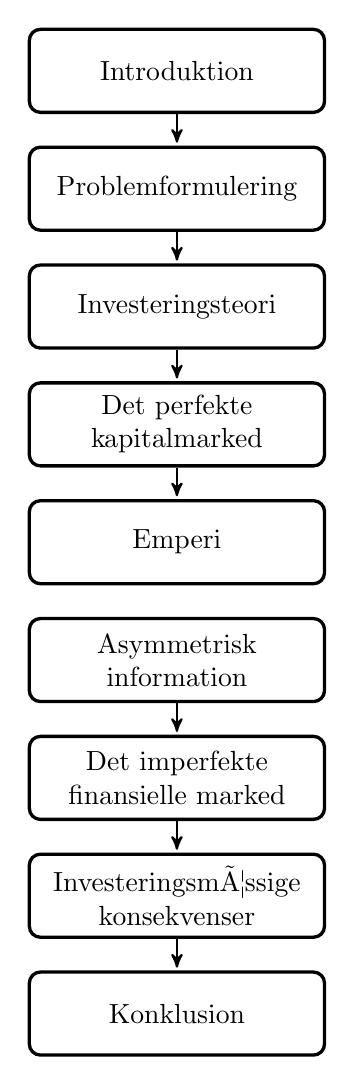
\begin{tikzpicture}
            [node distance=.4cm,
            start chain=going below,]
               \node[punktchain, join] (intro) {Introduktion};
               \node[punktchain, join] (probf)      {Problemformulering};
               \node[punktchain, join] (investeringer)      {Investeringsteori};
               \node[punktchain, join] (perfekt) {Det perfekte kapitalmarked};
               \node[punktchain, join, ] (emperi) {Emperi};
                \node (asym) [punktchain ]  {Asymmetrisk information};
            \node[punktchain, join,] (disk) {Det imperfekte finansielle marked};
            \node[punktchain, join,] (makro) {Investeringsmæssige konsekvenser};
            \node[punktchain, join] (konk) {Konklusion};
            \end{tikzpicture}
    \end{center}

    \begin{table}[!h]
        \centering
        \caption{DELAY BOUND $\tau_{max}$ FOR $c = 0.5$}\label{tab1}
        \begin{tabular}{{l l|l l}}
        \toprule
        $\tau_{max}^{YueHan}$ & 3.69 & $\tau_{max}^{Fridman}$ & 1.14  \\
        \midrule
        $\tau_{max}^{He}$ & 3.67 &  $\tau_{max}$ & 4.7274 \\
        \hline
        $\tau_{max}^{Han}$ & 3.62 & $\tau_{max}^{analytical}$ & 4.7388  \\
        \bottomrule
        \end{tabular}
    \end{table}
    
    \begin{table}[!h]
        \centering
        \caption{DELAY BOUND $\tau_{max}$ FOR VARIOUS c}\label{tab1}
        \begin{tabular}{{l l|l l}}
        \toprule
        $\tau_{max}^{YueHan}$ & 3.69 & $\tau_{max}^{Fridman}$ & 1.14  \\
        \midrule
        $\tau_{max}^{He}$ & 3.67 &  $\tau_{max}$ & 4.7274 \\
        \hline
        $\tau_{max}^{Han}$ & 3.62 & $\tau_{max}^{analytical}$ & 4.7388  \\
        \bottomrule
        \end{tabular}
    \end{table}
\end{exmp}

\begin{exmp}
    Consider a neutral system(xia)
    \begin{equation}
        \begin{aligned}
            \begin{bmatrix}
                \dot{x}(t) \\
                z(t) \\
                y(t) 
            \end{bmatrix} & = \begin{bmatrix}
                A_{0} & 0 & 0\\
                0 & 0 & 0\\
                0 & 0 & 0
            \end{bmatrix}\begin{bmatrix}
                x(t) \\
                w(t) \\
                u(t) 
            \end{bmatrix} \\ 
            &+ \quad \begin{bmatrix}
                A_{1} & 0 &0 & E_{1}\\
                0 & 0 & 0 & 0\\
                0 & 0 & 0 & 0
            \end{bmatrix} \begin{bmatrix}
                x(t-\tau_{1}) \\
                w(t-\tau_{1}) \\
                u(t-\tau_{1}) \\
                \dot{x}(t-\tau_{1})
            \end{bmatrix}.\label{eq}
        \end{aligned}
    \end{equation}
    Subsystem 1:
    \begin{equation}
        \begin{aligned}
            &A_{0} =  \begin{bmatrix}
                1.8 & -0.3\\
                0 & 2.5\\
            \end{bmatrix}
            &A_{1} =  \begin{bmatrix}
                -1 & 0\\
                -1 & -1
            \end{bmatrix}\\
            &E_{1} =  \begin{bmatrix}
                0.5 & \quad 0\\
                0 & \quad 0.5\\
            \end{bmatrix}\\
        \end{aligned}
        \nonumber
    \end{equation}
    Subsystem 2:
    \begin{equation}
        \begin{aligned}
            &A_{0} =  \begin{bmatrix}
                1.8 & -0.3\\
                0 & 2.5\\
            \end{bmatrix}
            &A_{1} =  \begin{bmatrix}
                -1 & 0\\
                -1 & -1
            \end{bmatrix}\\
            &E_{1} =  \begin{bmatrix}
                0.5 & \quad 0\\
                0 & \quad 0.5\\
            \end{bmatrix}\\
        \end{aligned}
        \nonumber
    \end{equation}
    
$\tau(t)$,$r$,$h$,$\alpha_{1}$,$\alpha_{2}$,$\beta_{1}$,$\beta_{2}$
\begin{equation}
    \begin{aligned}
        &K_{1} =  \begin{bmatrix}
            1.8 & -0.3\\
            0 & 2.5\\
        \end{bmatrix}
        &K_{2} =  \begin{bmatrix}
            -1 & 0\\
            -1 & -1
        \end{bmatrix}
    \end{aligned}
    \nonumber
\end{equation}
Let h(t) = t
\begin{equation}
    \begin{aligned}
        \setlength{\arraycolsep}{0.9pt}
        N_{t}^{\sigma}
    \end{aligned}
    \nonumber
\end{equation}

\begin{equation}
    \begin{aligned}
        \setlength{\arraycolsep}{0.9pt}
        \eta^{h}_{1}(1,t) = \eta^{h}_{1}(2,t) 
    \end{aligned}
    \nonumber
\end{equation}

\begin{equation}
    \begin{aligned}
        \setlength{\arraycolsep}{0.9pt}
        \eta^{h}_{2}(1,t) 
    \end{aligned}
    \nonumber
\end{equation}

\begin{equation}
    \begin{aligned}
        \setlength{\arraycolsep}{0.9pt}
        \eta^{h}_{2}(2,t) 
    \end{aligned}
    \nonumber
\end{equation}

\end{exmp}


\section{Conclusion}
cite Delay-Dependent Stability for Load FrequencyControl System via Linear Operator Inequality 
\begin{equation}
    \begin{aligned}
        \setlength{\arraycolsep}{0.9pt}
        \mathcal{T}'^{*}\mathcal{H}\mathcal{A}'+\mathcal{A}'^{*}\mathcal{H}\mathcal{T}' \textless 0
    \end{aligned}
\end{equation}
$\bold{PROOF:}$ 
\begin{equation}
    \begin{aligned}
        \setlength{\arraycolsep}{0.9pt}
        \dot{V}(\bold{x}) &= <\mathcal{T}'\bold{x},\mathcal{H}\mathcal{T}'\bold{x}>_{Z} + <\mathcal{A}'\bold{x},\mathcal{H}\mathcal{T}'\bold{x}>_{Z} \\ &=<\bold{x},(\mathcal{T}'^{*}\mathcal{H}\mathcal{A}'+\mathcal{A}'^{*}\mathcal{H}\mathcal{T}')\bold{x}>_{Z}  
    \end{aligned}
\end{equation}
\section{References}
cite Delay-Dependent Stability for Load FrequencyControl System via Linear Operator Inequality 
\begin{equation}
    \begin{aligned}
        \setlength{\arraycolsep}{0.9pt}
        \mathcal{T}'^{*}\mathcal{H}\mathcal{A}'+\mathcal{A}'^{*}\mathcal{H}\mathcal{T}' \textless 0
    \end{aligned}
\end{equation}
\begin{equation}
    \begin{aligned}
        \setlength{\arraycolsep}{0.9pt}
        \dot{V}(\bold{x}) &= <\mathcal{T}'\bold{x},\mathcal{H}\mathcal{T}'\bold{x}>_{Z} + <\mathcal{A}'\bold{x},\mathcal{H}\mathcal{T}'\bold{x}>_{Z} \\ &=<\bold{x},(\mathcal{T}'^{*}\mathcal{H}\mathcal{A}'+\mathcal{A}'^{*}\mathcal{H}\mathcal{T}')\bold{x}>_{Z}  
    \end{aligned}
\end{equation}

\section{Appendixes}

\begin{pf}
lemma2:\\
    Given NDS form
    \begin{equation}
        \begin{aligned}
            \begin{bmatrix}
                \dot{x}(t) \\
                z(t) \\
                y(t) 
            \end{bmatrix} & = \begin{bmatrix}
                A_{0} & 0 & B_{2}\\
                0 & 0 & 0\\
                0 & 0 & 0
            \end{bmatrix}\begin{bmatrix}
                x(t) \\
                w(t) \\
                u(t) 
            \end{bmatrix} \\ 
            &+ \sum_{i=1}^{K}\begin{bmatrix}
                A_{i} & 0 & B_{2i} & E_{i}\\
                0 & 0 & 0 & 0\\
                0 & 0 & 0 & 0
            \end{bmatrix} \begin{bmatrix}
                x(t-\tau_{i}) \\
                w(t-\tau_{i}) \\
                u(t-\tau_{i}) \\
                \dot{x}(t-\tau_{i})
            \end{bmatrix}\\
        \end{aligned}
    \end{equation}
    assume that
    \begin{equation}
        \begin{aligned}
            v(t) &= \sum_{i = 1}^{K}C_{vi}r_{i}(t-\tau_{i})
        \end{aligned}
    \end{equation}
    then we get
    \begin{equation}
        \begin{aligned}
            \begin{bmatrix}
                \dot{x}(t) \\
                z(t) \\
                y(t) 
            \end{bmatrix} & = \begin{bmatrix}
                A_{0} & 0 & B_{2}\\
                0 & 0 & 0\\
                0 & 0 & 0
            \end{bmatrix}\begin{bmatrix}
                x(t) \\
                w(t) \\
                u(t) 
            \end{bmatrix} + Iv(t)\\
        \end{aligned}
    \end{equation}
    $I$ is a identity matrix,we define
    \begin{equation}
        \begin{aligned}
            I & = \begin{bmatrix}
                B_{v} \\
                D_{1v} \\
                D_{2v} 
            \end{bmatrix} \\
        \end{aligned}
    \end{equation}
    so that
    \begin{equation}
        \begin{aligned}
            \begin{bmatrix}
                \dot{x}(t) \\
                z(t) \\
                y(t) 
            \end{bmatrix} & = \begin{bmatrix}
                A_{0} & 0 & B_{2}\\
                0 & 0 & 0\\
                0 & 0 & 0
            \end{bmatrix}\begin{bmatrix}
                x(t) \\
                w(t) \\
                u(t) 
            \end{bmatrix} + \begin{bmatrix}
                B_{v} \\
                D_{1v} \\
                D_{2v} 
            \end{bmatrix}v(t)\\
        \end{aligned}
    \end{equation}
    
    from the above eqution,we get
    \begin{equation}
        \begin{aligned}
                \dot{x}(t) 
            & = \begin{bmatrix}
                A_{0} & 0 & B_{2}
            \end{bmatrix}\begin{bmatrix}
                x(t) \\
                w(t) \\
                u(t) 
            \end{bmatrix} + 
                B_{v} v(t)\\
        \end{aligned}
    \end{equation}
    
    we can see $B_{v}v(t)$ Representing the first part of $v(t)$,so we get
    \begin{equation}
        \begin{aligned}
                B_{v} v(t) = \begin{bmatrix}
                    I & 0 & 0
                \end{bmatrix}v(t)
        \end{aligned}
    \end{equation}
    
    define 
    \begin{equation}
        \begin{aligned}
            r_{i}(t) = \begin{bmatrix}
                x(t) \\
                z(t) \\
                y(t) \\
                \dot{x}(t)
            \end{bmatrix} 
        \end{aligned}
    \end{equation}
    
    
    \begin{equation}
        \begin{aligned}
            r_{i}(t) &= \begin{bmatrix}
                x(t) \\
                z(t) \\
                y(t) \\
                \dot{x}(t)
            \end{bmatrix} = \begin{bmatrix}
                I & 0 & 0 \\
                0 & I & 0  \\
                0 & 0 & I  \\
                0 & 0 & 0 
            \end{bmatrix}\begin{bmatrix}
                x(t) \\
                w(t) \\
                u(t) 
            \end{bmatrix}+\begin{bmatrix}
                0 \\
                0 \\
                0 \\
                \dot{x}(t)
            \end{bmatrix}\\
            &= \begin{bmatrix}
                I & 0 & 0 \\
                0 & I & 0  \\
                0 & 0 & I  \\
                A_{0} & 0 & B_{2} 
            \end{bmatrix}\begin{bmatrix}
                x(t) \\
                w(t) \\
                u(t) 
            \end{bmatrix}+\begin{bmatrix}
                0 & 0 & 0 \\
                0 & 0 & 0\\
                0 & 0 & 0\\
                I & 0 & 0
            \end{bmatrix}v(t)
        \end{aligned}
    \end{equation}
    
    Cite [NDS to DDF] we get
    \begin{equation}
        \begin{aligned}
                r_{i}(t) & = \begin{bmatrix}
                C_{ri} & B_{r1i} & B_{r2i}
            \end{bmatrix}\begin{bmatrix}
                x(t) \\
                w(t) \\
                u(t) 
            \end{bmatrix} 
            + D_{rvi}v(t)
        \end{aligned}
    \end{equation}
    
    merge eqution (27) and eqution (30),we get the standard DDF form
    \begin{equation}
        \begin{aligned}
            \begin{bmatrix}
                \dot{x}(t) \\
                z(t) \\
                y(t) \\
                r_{i}(t)
            \end{bmatrix} & = \begin{bmatrix}
                A_{0} & 0 & B_{2}\\
                0 & 0 & 0\\
                0 & 0 & 0\\
                C_{ri} & B_{r1i} & B_{r2i}
            \end{bmatrix}\begin{bmatrix}
                x(t) \\
                w(t) \\
                u(t) 
            \end{bmatrix} + \begin{bmatrix}
                B_{v} \\
                D_{1v} \\
                D_{2v} \\
                D_{rvi}
            \end{bmatrix}v(t)\\
        \end{aligned}
    \end{equation}

\end{pf}

\begin{pf}
    lemma3:\\

\end{pf}
\end{document}


